% 左图按原始宽高比显示，三个采样点以左上角为原点，单位为像素。
\begin{tikzpicture}[x=1mm,y=1mm,
  every node/.style={font=\small\sffamily,text=Ink},
  tag/.style={circle,fill=Ink,draw=white,line width=.5pt,inner sep=1.5pt,text=white,font=\sffamily\bfseries\scriptsize}]
  \node[anchor=north west,inner sep=0] at (0,0)
    {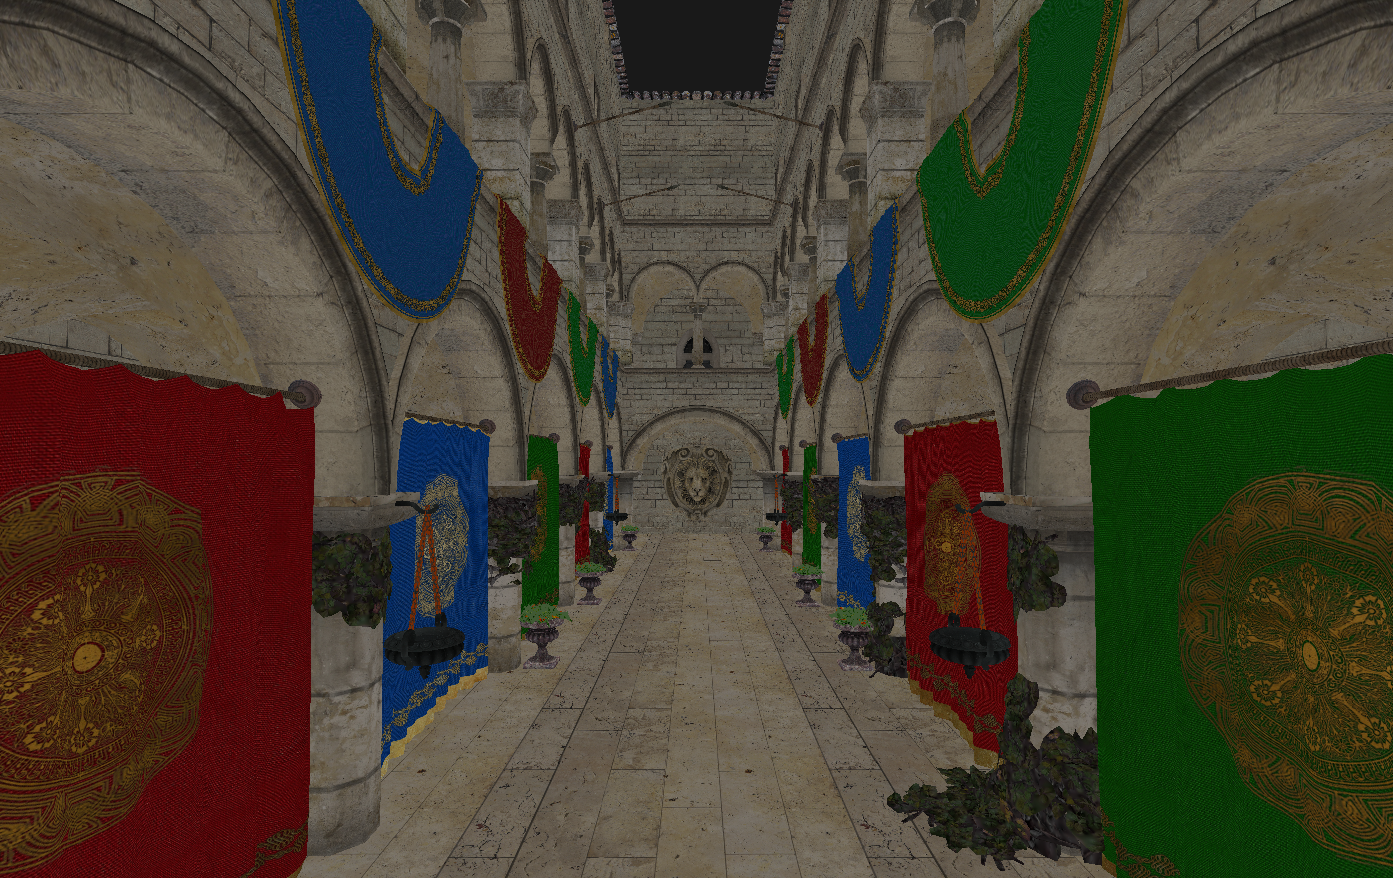
\includegraphics[width=91mm]{figures/sponza-picking.png}};
  \draw[Rule] (0,0) rectangle (91,{-91*(878/1393)});
  \foreach \x/\y/\id/\dx/\dy in {410/205/A/-6/-3,365/760/B/-7/4,690/40/C/8/-4}{
    \coordinate (sample) at ({91*((\x+0.5)/1393)},{-91*((\y+0.5)/1393)});
    \draw[Ink,line width=1.2pt] (sample)--++(\dx,\dy);
    \draw[white,line width=.55pt] (sample)--++(\dx,\dy) node[tag]{\id};
    \filldraw[fill=white,draw=Ink,line width=.45pt] (sample) circle (.75mm);
  }
  \foreach \y/\id/\what/\rgb/\value in {
    -6/A/蓝色挂毯/{29, 47, 87}/4,
    -25/B/石柱/{123, 116, 107}/4,
    -44/C/屋顶开口/{25, 25, 25}/$-1$}{
    \node[tag] at (98,\y){\id};
    \node[anchor=west,font=\sffamily\bfseries] at (102,\y){\what};
    \node[anchor=west,text=Muted] at (102,\y-5.1){RGB\enspace\rgb};
    \node[anchor=west,text=Teal] at (102,\y-10){实体编号\quad\value};
  }
\end{tikzpicture}
